\begin{Article}[Auteur={Gisèle Umbhauer\thanks{BETA, University of Strasbourg. \emph{Correspondence:} 61 Avenue de la Forêt Noire, 67085 Strasbourg Cedex, France. \emph{E-mail:}\href{mailto:umbhauer@unistra.fr}{\nolinkurl{umbhauer@unistra.fr}}}}, Titre={Minimax Regret in the 11-20 Money Request Game}]

\remerciementsEng{I thank two referees, as well as Jalal El Ouardighi and Bernardo Garcia-Pola for insightful comments. I also thank the third-year class students (year's class 2021/2022) at the Faculté des Sciences Economiques et de Gestion (Faculty of Economic and Management Sciences) of the University of Strasbourg, who played the 11--20 money request game.}

\begin{refsection}[Umbhauer]
\selectlanguage{english}

\begin{resumeENG}
Arad and Rubinstein's 11--20 money request game nicely triggers
level-\emph{k} reasoning. We show, in a general class of money-request games, that mixed-strategy minimax regret plays a significant role too, and that it mimics level-\emph{k} reasoning, at least if the number of level-\emph{k} players in a population is supposed to decrease in \emph{k}. We also show, in this class of games, an original link between the minimax regret probability distribution and the mixed-strategy Nash equilibrium distribution, and we compare the payoffs obtained with both concepts.
\end{resumeENG}

\titrearticleENG{Minimax regret et jeu de demande 11-20}

\begin{resume}
Le jeu de demande 11-20 d'Arad et Rubinstein stimule naturellement un comportement conforme au raisonnement de niveau-\emph{k}. Nous montrons, dans une version généralisée de ce jeu, que le minimax regret joue également un rôle significatif dans le comportement induit et que la stratégie mixte de minimax regret mime le raisonnement de niveau-\emph{k}, dès lors que le nombre de joueurs de niveau-\emph{k} dans une population chute avec \emph{k}. Nous montrons également qu'il existe, pour cette famille de jeux, un lien original entre la stratégie mixte de minimax regret et l'équilibre de Nash en stratégies mixtes, et nous comparons les paiements obtenus avec les deux concepts.
\end{resume}

\keywords{mixed minimax regret, level-\emph{k} reasoning, money-request game, Nash equilibrium}

\motscles{minimax regret en stratégies mixtes, raisonnement de niveau-\emph{k}, jeu de demande 11-20, équilibre de Nash}

\jelcode{C72}


\section{Introduction}

\textcite{arad2012} presented the 11--20 money request game
as the game that naturally triggers level-\emph{k} reasoning. In this
2-player game, each player requests an amount of money. This amount is an integer between 11 and 20. Each player receives the amount he asks for. And a player gets an additional amount of 20 if he requests exactly one unit less than the other player.

Arad and Rubinstein (AR henceforth) are partly right in claiming that
this game is well suited for studying level-\emph{k} reasoning. First, everything is done in this game to stimulate level-\emph{k} reasoning. The level-0 behavior seems to find consensus: by playing 20, a player is sure to get 20, which is a very large (unusual) maximin payoff. Hence a player who does not want to engage in iterative reasoning will surely request 20, so 20 is the natural starting point for the level-\emph{k} iterations. It follows that playing 19 is the natural level-1 behavior (because 19 is the best response to 20), that 18 is the natural level-2 behavior (because 18 is the best response to 19), and so on. Conflict between the two players is circumscribed in that each player gets the amount he asks for, regardless of what is played by the opponent, so individual optimization should not be limited by social considerations.

Second, the sequence of level-\emph{k} iterations cannot be obtained by other common ways of reasoning. There is no dominated strategy in the 11--20 money request game, so iterative dominance has no bite and cannot lead to the same outcome as level-\emph{k} behavior (by contrast to what happens in the guessing game (beauty contest), see \textcite{nagel1995}). There is also no pure strategy Nash equilibrium that is the limit behavior of level-\emph{k} reasoning (by contrast to the guessing game). Third, the game is very easy and requires few (almost no) cognitive skills to progress in the level-\emph{k} process. By contrast to guessing games where each additional step requires calculating a new mean, here each additional step consists just in decreasing the requested amount by 1; this fact explains why a slightly simplified version of Arad and Rubinstein's game (AR's game henceforth) has been used in experiments with very young children, from five years old (see \textcite{fe2022}). For all these reasons, the 11--20 money request game seems to be a good game to test level-\emph{k} reasoning, and especially the depth of reasoning (number of iterations performed by the players).

This game has given rise to many experiments (among them \textcite{arad2012}, \textcite{lindner2013}, \textcite{goeree2018}, \textcite{li2018}, \textcite{alosferrer2021}). Some of these studies have brought insights into time and depth of reasoning. \textcite{lindner2013} studied whether time pressure was able to stimulate a behavior closer to the mixed strategy Nash equilibrium, whereas \textcite{alosferrer2021} studied the link between deliberation times and depth of reasoning.

Yet AR's game has a property not shared by other level-\emph{k} testing
games like the usual guessing game. As observed by \textcite{li2018}, in contrast to the guessing game where the players always
get the same amount (1 for the winner and 0 for the losers), the payoff
obtained by a player in the money request game strongly depends on the
chosen number. The maximal and minimal amounts a player can win with a
given integer are increasing in the number played (except for 20): a
player gets at least 19 and at most 39 by playing 19 but only at least
11 and at most 31 by playing 11. This fact may trigger behavioral traits
that are different from level-\emph{k} reasoning. \textcite{li2018}
mention risk aversion, which indeed leads to players playing large
numbers more frequently, while \textcite{goeree2018} show that common
knowledge of noise in behavior also leads to large numbers being played
more often.

In this paper, we argue that minimax regret is another way to approach
the game. Minimax regret (MR henceforth) is well known in decision
theory, where it is associated with ambiguity aversion---and goes back
to \textcite{savage1951} and \textcite{niehans1948}---but it has only more
recently been introduced into game theory, notably by \textcite{linhart1989}, \textcite{renou2010} and \textcite{halpern2012}. As a matter of fact, the 11--20 money request game exhibits a strong strategic uncertainty: according to \textcolor{red}{Pearce's concept [1984]}, each amount is rationalizable (because each request \emph{x}
from 11 to 19 is the best response to the request \(x + 1\), and 20 is
the best response to the request 11). So it is difficult to anticipate
the other's behavior and each decision may generate a regret. It follows
that it may be more reasonable to minimize the generated regrets rather
than trying to best respond to a strategy that cannot be anticipated.
And it turns out that the mixed MR strategy corresponds to the outcome
distribution observed with level-\emph{k} players, up to a certain depth
of reasoning, provided one assumes that the number of players in a
population is decreasing in the depth of reasoning. So level-\emph{k}
behavior can also be obtained by regret minimization despite its
conveying a completely different philosophy. \textcite{garciapola2020} already observed a link between level-1 reasoning and iterative pure-strategy MR. But pure-strategy MR only focuses on maximal regrets, which is very restrictive. Mixed-strategy MR better exploits all the regrets in the game and leads to a more interesting link between MR and level-\emph{k} reasoning.

The aim of this paper is to investigate the link between mixed-strategy
MR and level-\emph{k} reasoning, as well as the link between
mixed-strategy MR and the mixed-strategy Nash equilibrium in a general
version of the 11--20 money request game. We also compare the payoffs
obtained with MR and the Nash equilibrium. Finally we show how MR
behaves in variants of the 11--20 money request game developed by \textcite{arad2012} and \textcite{goeree2018}, and we make some behavioral
comments drawing on a classroom experiment.

In section~\ref{section:The 11-20 money} we start by briefly showing how 410 students played the 11--20 money request game in a classroom experiment at Strasbourg
university. This classroom experiment will be used to illustrate the
results set out in the following sections. In section~\ref{section:Minimax regret in the money} we establish the mixed-strategy MR regret behavior in the 11--20 money request game, before looking for this behavior in a general money request game. We
show that the mixed MR strategy mimics an outcome distribution of
level-\emph{k} players, if the percentage of players is decreasing in
the depth of reasoning. In section~\ref{section:Minimax regret, Nash equil} we study the original link between the mixed MR strategy and the mixed-strategy Nash equilibrium in the money request games, and we discuss the payoffs obtained with both
concepts. Section~\ref{section:Comments on minimax regrets} investigates the impact of MR in some variants of AR's game. Section~\ref{section:Conclusion_Umbhauer_en} concludes with behavioral comments drawing on the classroom experiment in Strasbourg.


\section[The 11-20 money request game, a classroom experiment]{The 11-20 money request game,\\ a classroom experiment}
% entre crochets le titre tel qu'il serait imprimé en table des matières ou en tête de page si c'était le cas
% entre accolades, le titre tel qu'on veut l'afficher dans le corps du texte
\label{section:The 11-20 money}

The classroom experiment was run during a third-year class in game
theory at the faculty of economics and management of the University of
Strasbourg in the academic year 2021--2022. In total 410 students
participated in the experiment. Subjects were homogeneous in age (almost
all students were 19--21~years old) and field of study (economics and
management). As is common in classroom experiments, no monetary rewards
were used to incentivize subjects but students were told that they could
obtain a bonus in the final grade for their participation in the
experiment. The experiment is a one-shot AR's game. The game was
explained and several examples were given to the students before the
beginning of the experiment, to be sure that the rules of the game were
understood.\footnote{To facilitate the understanding of the game we
  talked about amounts in euros (in \textcite{arad2012} the amounts are in
  shekels).} The students played the game before knowing the concepts of
dominance and Nash equilibrium (NE), but they knew the notion of a
normal form matrix game. So, when taking their decision, they had in
front of them the normal form matrix of the 11--20 money request game
(matrix 1).\footnote{To facilitate the reading of the matrix, player 1's
  payoffs were written in red. In the other experiments with the 11--20
  money request game, the players usually do not have the payoff matrix
  in front of them. Yet having the matrix at one's disposal may have an
  impact on the choices in that it facilitates the comparison of one's
  own payoff with the payoff of the opponent (we come back to this fact
  in section~\ref{section:Conclusion_Umbhauer_en}).}

\begin{table}[h!]
\centering
Matrix 1: The 11-20 money request game with bonus~20
\label{matx1}
\resizebox{.90\linewidth}{!}{
\begin{tabular}{lc | c*{9}{c} | }
\multicolumn{12}{c}{P12} \tabularnewline % fusionner 12 cellules, centrer (c)
 & \multicolumn{1}{c}{} & 11 & 12 & 13 & 14 & 15 & 16 & 17 & 18 & 19 & \multicolumn{1}{c}{20} \tabularnewline
\cline{3-12}
& 11 & (11,11) & (31,12) & (11,13) & (11,14) & (11,15) & (11,16) &
(11,17) & (11,18) & (11,19) & (11,20) \tabularnewline
& 12 & (12,31) & (12,12) & (32,13) & (12,14) & (12,15) & (12,16) &
(12,17) & (12,18) & (12,19) & (12,20) \tabularnewline
& 13 & (13,11) & (13,32) & (13,13) & (33,14) & (13,15) & (13,16) &
(13,17) & (13,18) & (13,19) & (13,20) \tabularnewline
& 14 & (14,11) & (14,12) & (14,33) & (14,14) & (34,15) & (14,16) &
(14,17) & (14,18) & (14,19) & (14,20) \tabularnewline
Pl1 & 15 & (15,11) & (15,12) & (15,13) & (15,34) & (15,15) & (35,16) &
(15,17) & (15,18) & (15,19) & (15,20) \tabularnewline
& 16 & (16,11) & (16,12) & (16,13) & (16,14) & (16,35) & (16,16) &
(36,17) & (16,18) & (16,19) & (16,20) \tabularnewline
& 17 & (17,11) & (17,12) & (17,13) & (17,14) & (17,15) & (17,36) &
(17,17) & (37,18) & (17,19) & (17,20) \tabularnewline
& 18 & (18,11) & (18,12) & (18,13) & (18,14) & (18,15) & (18,16) &
(18,37) & (18,18) & (38,19) & (18,20) \tabularnewline
& 19 & (19,11) & (19,12) & (19,13) & (19,14) & (19,15) & (19,16) &
(19,17) & (19,38) & (19,19) & (39,20) \tabularnewline
& 20 & (20,11) & (20,12) & (20,13) & (20,14) & (20,15) & (20,16) &
(20,17) & (20,18) & (20,39) & (20,20) \tabularnewline
\cline{3-12}
\end{tabular}}
\end{table}

  
The students had to answer the following question: ``Imagine you
are player~1 and you are confronted with another student, player~2,
randomly selected from all the other students. What amount do you ask
for?'' The students were invited to justify their choices in writing.
The results are given in table 1 and represented in figure 1. Table 1
also gives the results obtained in the experiments by AR {[}2012{]} and \textcite{li2018} (LR henceforth), as well as the mixed-strategy
symmetric NE,\footnote{The 11--20 money request game has other
  asymmetric mixed-strategy Nash equilibria, but they all meet the
  property that the probabilities on the played actions decrease in the
  played numbers, with a possible exception for the lowest played
  number. One of these equilibria is such that one player plays 13, 15,
  17, 19, respectively with the probabilities 8/20, 6/20, 4/20 and 2/20,
  whereas the other plays 12, 14, 16, 18 and 20, respectively with the
  probabilities 2/20, 7.5/20, 5.5/20, 3.5/20 and 1.5/20.} and the mixed
MR strategy we turn to in section~\ref{section:Minimax regret in the money}.

\begin{table}[h!]
\caption{Some experiments on the 11--20 money request game with
bonus 20, as well as the symmetric mixed Nash equilibrium and the mixed
minimax regret strategy}\label{tab1}
\centering
\resizebox{\linewidth}{!}{
\begin{tabular}{l    *{10}{D{6mm}}}
\toprule
Requested amount & \centering 11 & \centering 12 & \centering 13 & \centering 14 & \centering 15 & \centering 16 & \centering 17 & \centering 18 & \centering 19 & \centering 20 \tabularnewline
\midrule
Strasbourg's experiment (\%) & 8.3 & 0.7 & 2 & 4.4 & 4.9 & 5.9 & 14.9 &
17.5 & 28 & 13.4 \tabularnewline
AR's experiment (\%) & 4 & 0 & 3 & 6 & 1 & 6 & 32 & 30 & 12 & 6 \tabularnewline
LR's experiment (\%) & 0 & 0 & 0 & 7.3 & 1 & 4.2 & 19.8 & 37.5 & 26 &
4.2 \tabularnewline
Symmetric NE (\%) & 0 & 0 & 0 & 0 & 25 & 25 & 20 & 15 & 10 & 5 \tabularnewline
Mixed MR strategy (\%) & 0 & 0 & 0 & 0 & 5 & 10 & 15 & 20 & 25 & 25 \tabularnewline
\bottomrule
\end{tabular}}
\end{table}


\begin{figure}[h]
    \centering
    \caption{Strasbourg University's classroom experiment (percentages) (2021/2022)}
    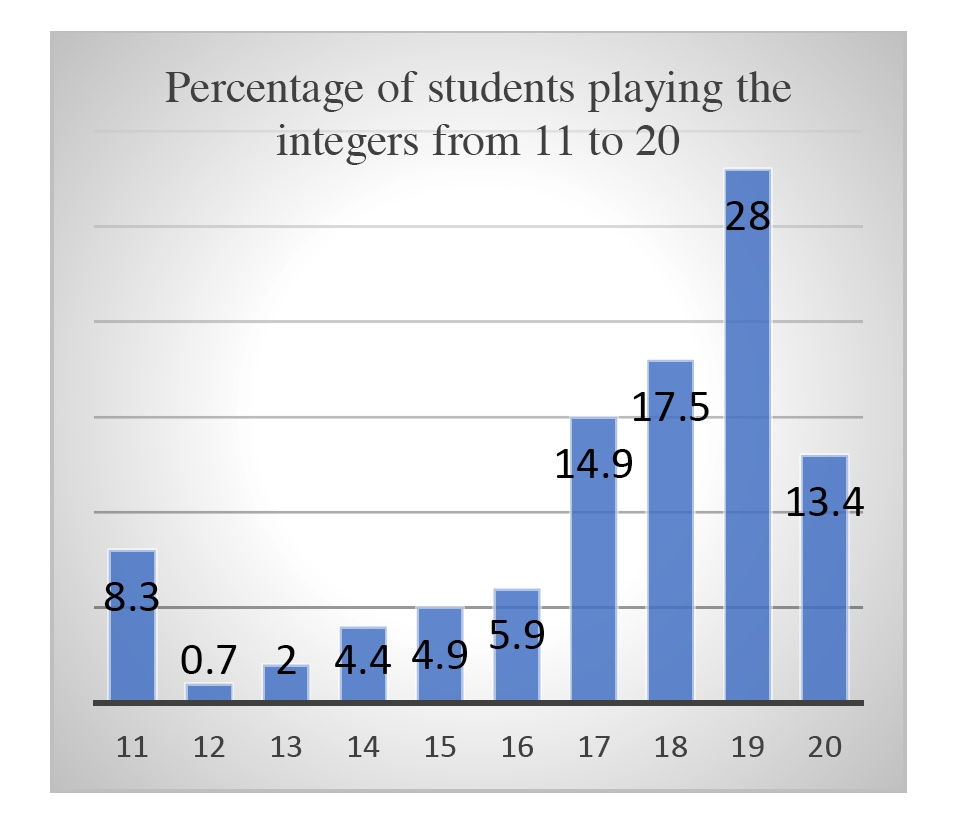
\includegraphics[height=7cm]{Articles-bons-a-composer/07_Umbhauer_en/07_Umbhauer_en_figures/Umbhauer_fig1.jpeg}
\end{figure}


Figure 1 is in line with a common observation made in many games
triggering level-\emph{k} behavior, namely guessing games (beauty
contests), according to which the number of players engaging in
level-\emph{k} reasoning is decreasing in the depth of reasoning
(\(k > 0\)). So 28\% of the students in Strasbourg choose 19 (level-1
reasoning), 17.5\% of them play 18 (level-2 reasoning), 14.9\% of them
play 17 (level-3 reasoning) and so on, down to 12 (see table 1). Only
the fact that 8.3\% of the students play 11 is not in accordance with
this fact. This smooth decreasing relationship from 19 to 12 is not
always obtained in other experiments on the 11--20 money request game.
19 is not always the statistical mode of the behavior distribution: 19
is the statistical mode in \textcolor{red}{Alos-Ferrer and Buckenmaier [2018]}, 17 is
the statistical mode in AR {[}2012{]}, and 18 is the statistical mode in \textcite{goeree2018}, \textcite{li2018} and \textcite{lindner2013}. More generally, the behavior distributions vary among the studies,\footnote{For example, a chi-square test on the populations, even if restricted to the distributions on the range 16--19, shows that AR's distribution (108 players) is statistically significantly different from the distribution obtained in the Strasbourg classroom experiment (410 players) (\emph{p}-value~<~0.001). Strasbourg's
  distribution is closer to the one obtained in \textcolor{red}{Alos-Ferrer and  Buckenmaier {[}2018{]}} (128 players), except for the number of players
  playing 17, which is quite low in Alos-Ferrer and Buckenmaier: both
  distributions, when restricted on the numbers 16, 18, 19 and 20, are
  not statistically significantly different (\(p = 0.14\)).} but all the
experiments share the property that the percentages decrease from 18 (17
for AR) to at least 14 (in any case, the percentages of players choosing
11, 12, 13 are generally small). And all the empirical distributions are
markedly different from the symmetric NE (the \emph{p}-value of the
chi-square tests can be approximated by 0).

\section{Minimax regret in the money request games}
\label{section:Minimax regret in the money}

We now turn to MR and apply this concept to a generalized version of
AR's game, the 11--\emph{T} money request game with bonus \emph{B}, with
\(B \geq T > 11 + n\), where \emph{n} is the integer defined by:
\(n(n + 1)/2\  \leq B < (n + 1)(n + 2)/2\) (\(B = T = 20\) and \(n = 5\)
in AR's game).

The notion of MR is well known in decision theory with uncertainty,
going back to \textcite{savage1951} and \textcite{niehans1948}. An economic
agent who is unable to anticipate a future state of the world (state of
Nature) may opt for a strategy that minimizes his regret, which is the
difference between the payoff obtained with his decision and the payoff
obtained with the best decision in the realized state of the world. MR
can partly explain the behavior of the agents in Ellsberg's paradox
\parencite{ellsberg1961}. In a game, players are not confronted with Nature or
lotteries---at least not exclusively---but with other players. Yet they
may also suffer from a strong strategic uncertainty, in that it may be
difficult, for many reasons, to anticipate how the other players will
play. In such a context, minimizing regrets may be more optimal than
best-replying to a completely unknown profile of strategies.

In a game, the pure-strategy MR concept goes as follows: in a
normal-form game with \emph{N} players \emph{i}, pure strategy sets
\emph{S\textsubscript{i}} and utility functions
\emph{u\textsubscript{i}}, with \emph{i} from 1 to \emph{N}, player
\emph{i}'s regret by playing the pure strategy \(s_{i}\ \)when the
opponents play the pure strategies \(s_{- i}\) is
\(r_{i}(s_{i}, s_{- i}) = \max_{\sigma_{i} \in S_{i}}{u_{i}\left( \sigma_{i}, s_{- i} \right) - u_{i}\left( s_{i}, s_{- i} \right)}\).
The maximal regret \emph{s\textsubscript{i}} leads to is
\(R_{i}\left( s_{i} \right) = \max_{s_{- i} \in S_{- i}}{r_{i}(s_{i}, s_{- i})}\).
Player \emph{i}'s pure-strategy MR is
\(\min_{s_{i} \in S_{i}}{R_{i}\left( s_{i} \right)}\) (see \textcite{linhart1989}, \textcite{halpern2012} and \textcite{renou2010} for more details).

Hence the regret generated by a chosen strategy, given an opponent's
strategy, is the difference between the payoff obtained with the
best-reply to the opponent's strategy and the payoff obtained with the
chosen strategy. For example, in the 11--20 money request game, if
player 1 asks for 14 whereas player 2 asks for 17, player 1's best
response is 16, and so player~1's regret, \emph{r}(14,17), is
$36-14=22$. The maximal regret the amount 14 may lead to,
\emph{R}(14), is obtained when player~2 chooses 20, in which case the
best response is 19 and the maximal regret generated by 14 is $39-14=25$.

The regret matrix for player 1 in AR's game is matrix 2. The maximal
regret assigned to each amount \emph{m}, \(R(m),\ m\) from 11 to 20, is
in bold in the matrix.

This matrix sheds light on the characteristics of the regrets. The
regrets in italics, equal to 19, express the fact that if both players
request \emph{x}, each player regrets not requesting \(x - 1\): he would
receive the additional amount \(B - 1\) by doing so (\emph{B} being the
bonus equal to 20 in AR's game). The regrets in the last column are the
regrets a player suffers when he plays \emph{x} different from 19 and
the opponent plays 20. The lower the requested amount \emph{x}, the more
he suffers, because he suffers both from the loss of the bonus 20 and
from the difference \(19 - x\).

\begin{table}[h!]
\centering
Matrix 2: Player 1's regret matrix in the 11--20 money request game\\ with bonus~20 \par
\vspace{0.2cm}
\label{matx2}
\resizebox{.55\linewidth}{!}{
\begin{tabular}{lc | c*{9}{c} | }
\multicolumn{12}{c}{P12} \tabularnewline
& \multicolumn{1}{l}{} & 11 & 12 & 13 & 14 & 15 & 16 & 17 & 18 & 19 & \multicolumn{1}{l}{20} \tabularnewline
\cline{3-12}
& 11 & 9 & 0 & 21 & 22 & 23 & 24 & 25 & 26 & 27 & \textbf{28} \tabularnewline
& 12 & 8 & \emph{19} & 0 & 21 & 22 & 23 & 24 & 25 & 26 & \textbf{27} \tabularnewline
& 13 & 7 & 18 & \emph{19} & 0 & 21 & 22 & 23 & 24 & 25 & \textbf{26} \tabularnewline
& 14 & 6 & 17 & 18 & \emph{19} & 0 & 21 & \emph{22} & 23 & 24 & \emph{\textbf{25}} \tabularnewline
Pl1 & 15 & 5 & 16 & 17 & 18 & 19 & 0 & 21 & 22 & 23 & \textbf{24} \tabularnewline
& 16 & 4 & 15 & 16 & 17 & 18 & \emph{19} & 0 & 21 & 22 & \textbf{23} \tabularnewline
& 17 & \ul{3} & \ul{14} & \ul{15} & \ul{16} & \ul{17} & \ul{18} &
\emph{\ul{19}} & \ul{0} & \ul{21} & \textbf{\ul{22}} \tabularnewline
& 18 & \ul{2} & \ul{13} & \ul{14} & \ul{15} & \ul{16} & \ul{17} &
\ul{18} & \emph{\ul{19}} & \ul{0} & \textbf{\ul{21}} \tabularnewline
& 19 & 1 & 12 & 13 & 14 & 15 & 16 & 17 & 18 & \emph{\textbf{19}} & 0 \tabularnewline
& 20 & 0 & 11 & 12 & 13 & 14 & 15 & 16 & 17 & 18 & \emph{\textbf{19}}
\tabularnewline
\cline{3-12}
\end{tabular}}
\end{table}


The matrix is quite regular in structure. On line \emph{x} (the amount
requested by player 1) the regrets are increasing in the opponent's
(player 2) amount \emph{y} up to \(y = x\), and they increase again in
player 2's amount \emph{y} from \(y = x + 2\) to \(y = 20\). Except for
\(x = 19,\) the maximal regret \(R(x)\) is always obtained in the last
column, when the opponent plays 20. This is due to the fact that the
regret in this column, except for 0, is \(B + 19 - x,\) whereas in
column \emph{y}, with \(11 < y < 20\), it is \(B + y - 1 - x\), which is
lower by construction.

\textcite{garciapola2020} observed that the pure-strategy MR in this game,
equal to 19, is obtained for \(x = 19\) and \(x = 20\), and that
applying the pure-strategy MR concept in an iterative way \parencite{halpern2012} leads to 19. By comparing MR with level-\emph{k} reasoning,
he concluded that, in this game, MR and level-1 reasoning lead to
requesting the same amount, 19.

In this paper we go further by turning to mixed-strategy MR, a concept
that takes into account all the regrets in matrix 2 (and not only the
maximal---bold--- regrets). We call \emph{x}, respectively \emph{y}, the
amounts played by player 1, respectively player 2 (the opponent). The
regrets in any line \emph{x} are regularly increasing in the opponent's
amount \emph{y} because they are equal to \(y - 1 + B - x\ \)(except for
\(y = x + 1\)). Comparing adjacent lines \emph{x} and \(x + 1\) (for
example the underlined lines 17 and 18) leads us to observe that player
1's regrets are always lower in line \(x + 1\) than in line \emph{x},
except if the other player plays \(x + 1\) (in this case, player 1's
regret is null when he plays \emph{x} and equal to 19 when he plays
\(x + 1\)). This fact expresses that a player regrets the unit of money
he deliberately and systematically loses when he plays \emph{x} instead
of \(x + 1\), except if the other player fortunately plays \(x + 1\).
Similar observations can be made by comparing two adjacent columns,
\emph{y} and \(y + 1\) (for example the squared columns 17 and 18). This
time the regrets are systematically one unit larger in column \(y + 1\)
than in column \emph{y}, because they switch from \(B + y - 1 - x\) to
\(B + y - x\). The regrets in column \emph{y}, i.e. when the opponent
plays \emph{y}, are regularly decreasing in \emph{x} (except for
\(x = y - 1\)). This follows from the fact that the regret
\(B + y - 1 - x\ \)can be split into two parts: the regret player 1
suffers when he plays 20, \(y - 1 + B - 20\), plus the regret he suffers
because he does not play 20, \(20 - x\), except for \(x = y - 1\). So
the regrets in column \emph{y} are decreasing in \emph{x} because
\(20 - x\) is decreasing in \emph{x}.

This intuitively leads to the following expectation: a concept of regret
should assign a stronger probability to larger numbers. This expectation
is revealed to be correct.

We work with \textcite{renou2010} mixed notion of regret. The
idea is to construct a mixed strategy that minimizes the regret, called
\emph{z}, regardless of the amount requested by the opponent. We call
\emph{p\textsubscript{t}} player 1's probability of requesting \emph{t}.
This amounts to solving the optimization program:
%
\[
\min_{z\ p_{11}p_{12}p_{13}p_{14}p_{15}p_{16}p_{17}p_{18}p_{19}p_{20}}z
\]
u.c.
\begin{multline}
9p_{11} + 8p_{12} + 7p_{13} + 6p_{14} + 5p_{15} + 4p_{16} + 3p_{17} + 2p_{18} + 1p_{19} + 0p_{20} \leq z \\
0p_{11} + 19p_{12} + 18p_{13} + 17p_{14} + 16p_{15} + 15p_{16} + 14p_{17} + 13p_{18}
+ 12p_{19} + 11p_{20} \leq z \\
21p_{11} + 0p_{12} + 19p_{13} + 18p_{14} + 17p_{15} + 16p_{16} + 15p_{17} + 14p_{18}
+ 13p_{19} + 12p_{20} \leq z \\
22p_{11} + 21p_{12} + 0p_{13} + 19p_{14} + 18p_{15} + 17p_{16} + 16p_{17} + 15p_{18}
+ 14p_{19} + 13p_{20} \leq z \\
23p_{11} + 22p_{12} + 21p_{13} + 0p_{14} + 19p_{15} + 18p_{16} + 17p_{17} + 16p_{18}
+ 15p_{19} + 14p_{20} \leq z \\
24p_{11} + 23p_{12} + 22p_{13} + 21p_{14} + 0p_{15} + 19p_{16} + 18p_{17} + 17p_{18}
+ 16p_{19} + 15p_{20} \leq z \\ \tag{1}
25p_{11} + 24p_{12} + 23p_{13} + 22p_{14} + 21p_{15} + 0p_{16} + 19p_{17} + 18p_{18}
+ 17p_{19} + 16p_{20} \leq z \\
26p_{11} + 25p_{12} + 24p_{13} + 23p_{14} + 22p_{15} + 21p_{16} + 0p_{17} + 19p_{18}
+ 18p_{19} + 17p_{20} \leq z \\
27p_{11} + 26p_{12} + 25p_{13} + 24p_{14} + 23p_{15} + 22p_{16} + 21p_{17} + 0p_{18}
+ 19p_{19} + 18p_{20} \leq z \\
28p_{11} + 27p_{12} + 26p_{13} + 25p_{14} + 24p_{15} + 23p_{16} + 22p_{17} + 21p_{18}
+ 0p_{19} + 19p_{20} \leq z \\
p_{11} + p_{12} + p_{13} + p_{14} + p_{15} + p_{16}{+ p}_{17} + p_{18} + p_{19} + p_{20} = 1 \\
0 \leq p_{t}\enskip \text{from 11 to 20.}
\end{multline}

Solving this program leads to the probabilities $p_{i} = 0$, $i$ from 11 to 14, $p_{15} = \frac{1}{20}, p_{16} = \frac{2}{20}, p_{17} = \frac{3}{20}, p_{18} = \frac{4}{20}, p_{19} = \frac{5}{20}, p_{20} = \frac{5}{20}$. The MR is $z=315/20=15.75$. This distribution is illustrated in figure~2 and table~1. By comparing figure~1 and figure~2, we observe that the students' behavior in the Strasbourg classroom experiment fits well with the MR distribution, with exception of \emph{p}\textsubscript{20} and \emph{p}\textsubscript{11} which are respectively much lower and much larger than 5/20 and 0. This is confirmed by a chi-square test: when we focus on the range 15--19, the
experimental distribution is not statistically significantly different
from the distribution obtained with 410~players playing the mixed MR
strategy (\emph{p}-value =~0.25). By contrast, obviously, the
experimental distribution is significantly different from the Nash
distribution (the \emph{p}-value can be approximated by 0 even if we
focus on a limited range of integers).

The result obtained for AR's game generalizes to the 11--\emph{T} money
request game, with a bonus \emph{B}, with \(B \geq T > 11 + n\), where
\emph{n} is the integer defined by:
\(n(n + 1)/2\  \leq B < (n + 1)(n + 2)/2\).

% FIGURE 2

\begin{figure}[h]
    \centering
    \caption{Mixed minimax regret strategy in AR's game}
    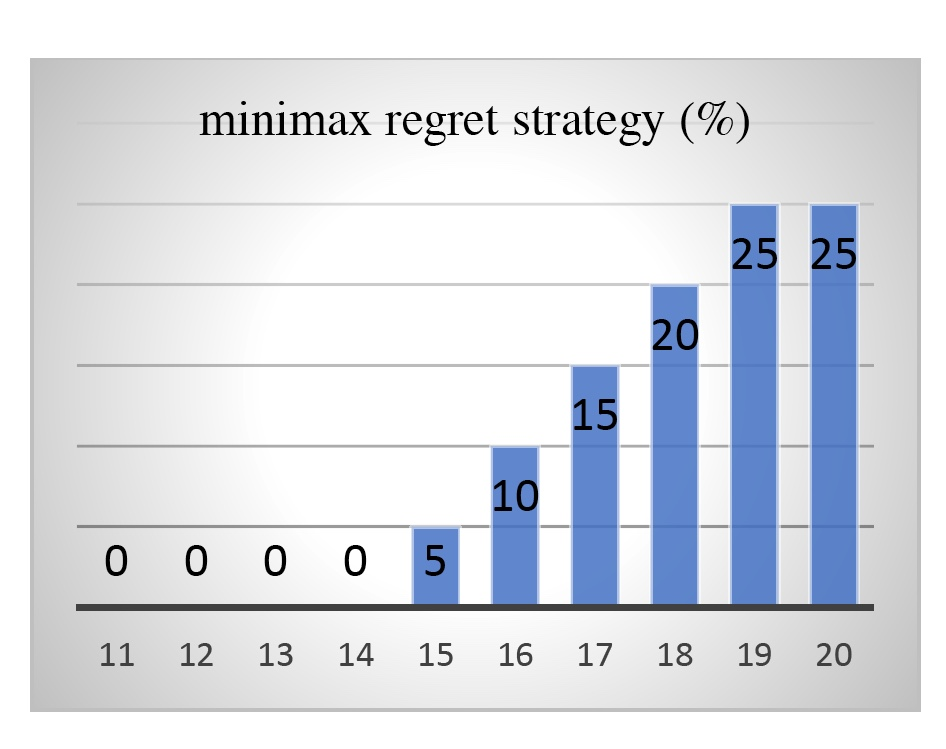
\includegraphics[height=5cm]{Articles-bons-a-composer/07_Umbhauer_en/07_Umbhauer_en_figures/Umbhauer_fig2.jpeg}
\end{figure}

% FIGURE 3

\begin{figure}[h]
    \centering
    \caption{Mixed-strategy symmetric Nash Equilibrium in AR's game}
    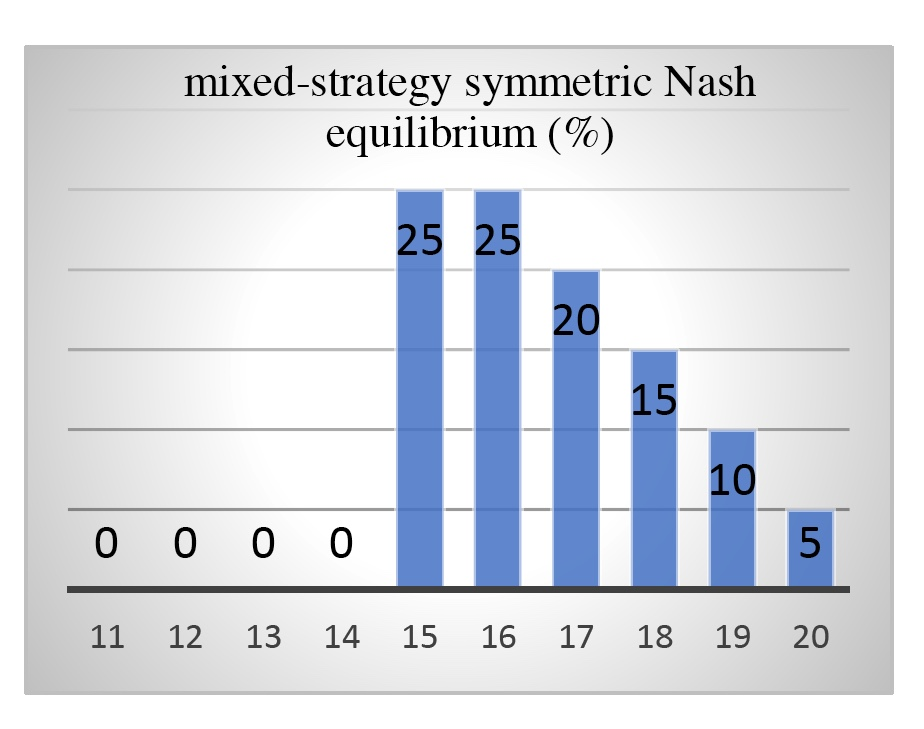
\includegraphics[height=5cm]{Articles-bons-a-composer/07_Umbhauer_en/07_Umbhauer_en_figures/Umbhauer_fig3.jpeg}
\end{figure}

\clearpage

% PROPOSITION 1

\begin{proposition}

a) In the 11--T money request game with bonus B, \(B \geq T > 11 + n\), n being the integer defined by \(\frac{n(n + 1)}{2} < B < \frac{(n + 1)(n + 2)}{2}\), the mixed
MR strategy is given by:

{\centering
\(p_{i} = 0\), i from 11 to T--n--1 \\
\(p_{T - n + i} = \frac{i + 1}{B}\), i from 0 to n--1 \\
\(p_{T} = 1 - \frac{n(n + 1)}{2B}\);\par}

b) For \(B \geq T > 11 + n\) and \(B=\frac{n(n + 1)}{2}\), the mixed MR strategies are the convex combinations of the following two distributions:

{\centering
$p_{i} = 0$, i from 11 to $T-n-1$, \\
$p_{T - n + i} = \frac{i + 1}{B}$, i from 0 to $n-1$, \\
$p_{T} = 0$,\par}

and

{\centering
$p_{i} = 0$, i from 11 to $T-n$, \\
$p_{T - n + i} = \frac{i}{B}$, i from 1 to n;\par}

c) The MR, z, is equal to
\(B + \frac{n(n + 1)(n + 2)}{6B}\ –\ (n + 1)\).
\end{proposition}

\begin{proof}
   See appendix~\ref{Annexe:Proof of Prop 1}. \quad \blacksquare 
\end{proof}

\vspace{0.5cm}
\emph{a}) is illustrated by AR's game, with \(T = B = 20\) and \(n = 5\).
\emph{b}) is illustrated for \(B = T = 21\) and \(n = 6\). Two distributions,

{\centering \(p_{i} = 0\) for \emph{i} from 11 to 14,
$p_{15} = \frac{1}{21}, p_{16} = \frac{2}{21}, p_{17} = \frac{3}{21}, p_{18} = \frac{4}{21}$,\par}

{\centering \(p_{19} = \frac{5}{21}, p_{20} = \frac{6}{21}, p_{21} = 0\)\par}

\noindent and

{\centering $p_{i} = 0$ for \emph{i} from 11 to 15,
$p_{16} = \frac{1}{21}, p_{17} = \frac{2}{21}, p_{18} = \frac{3}{21}, p_{19} = \frac{4}{21}$,\par} 

{\centering $p_{20} = \frac{5}{21}, p_{21} = \frac{6}{21}$,\par}

\noindent lead to the minimal regret 50/3, and any convex combination of both
distributions also leads to the minimal regret.

Proposition 1 gives rise to the following comments.

When \(\frac{n(n + 1)}{2} < B,\) \emph{p\textsubscript{T}}
(\emph{p}\textsubscript{20} in AR's game) is just the complement to 1 of
the sum \(\sum_{i = T - n}^{T - 1}p_{i}\). In AR's game,
\emph{p\textsubscript{T}} = \emph{p\textsubscript{T--1 }}= 5/20: so, by
construction, the probability assigned to the highest amount (that
corresponds to the level-0 reasoning) is lower than or equal to the
probability assigned to the amount \(T - 1\) (the level-1 reasoning
amount).

Proposition 1 shows that for \(B > \frac{n(n + 1)}{2}\),
\emph{p\textsubscript{i}} is linearly increasing in \emph{i}, with
\emph{i} from \(T - n\) to \(T - 1\):
$p_{T - n} = \frac{1}{B}$, $p_{T - 1} = \frac{n}{B}$ and $p_{i} - p_{i - 1} = 1/B$.
For \(B = \frac{n(n + 1)}{2}\), \emph{p\textsubscript{i}} is also
increasing in \emph{i}, with \emph{i} from \(T - n\) to \(T - 1\), but
\emph{p\textsubscript{T}} can be larger than, lower than, or equal to
\emph{p\textsubscript{T--1}}.

These increasing probabilities are in line with previous expectations: a
player always regrets not playing \(y - 1\), where \emph{y} is the
amount played by the opponent, but this regret is decreasing in the
amount \emph{x} he plays, because \(y - 1 + B - x\) is decreasing in
\emph{x}.

Proposition 1 goes beyond \textcite{garciapola2020}'s result. This author showed that the iterative pure-strategy MR reasoning fits
with level-1 reasoning, which consists in requesting the amount 19 in
AR's game. Proposition 1 shows that the mixed MR strategy fits with a
level-\emph{k} outcome distribution, from level-1 to level-\emph{n},
when each additional step of reasoning is achieved by fewer persons. So,
in the 11--20 money request game with bonus 20, the MR probabilities fit
with the outcome distribution observed with level-\emph{k} players when
25\% of the players do a level-1 reasoning (hence play 19), 20\% do a
level-2 reasoning (i.e. play 18), 15\% do a level-3 reasoning (i.e. play
17), 10\% do a level-4 reasoning (i.e. play 16) and 5\% do a level-5
reasoning (i.e. play 15). So, despite MR having nothing to do with
level-\emph{k} reasoning, it selects a similar behavior in the
11--\emph{T} money request game with bonus \emph{B}, at least if one
assumes that the percentage of players able to do a level-\emph{k}
reasoning is decreasing in \emph{k}. Given that \emph{p\textsubscript{i}
=} 0 for \(i < T - n\), this result, to be compatible with
level-\emph{k} reasoning, requires that nobody is able to do a
level-(\emph{n+1}) (i.e. deeper) reasoning. \(B \geq T > 11 + n\) and
\(B > n(n + 1)/2\) imply \(n \geq 5\), so this limited depth of
reasoning is not very restrictive, in that in reality people seldom do
more than a level-4 reasoning (see for example \textcite{crawford2013}). To
put it more exactly, even if able to make more than 4 steps of
level-\emph{k} reasoning, people often refrain from doing so in that
they fear that the other players are not able to do so.\footnote{So it
  is one's theory of mind, the ability to enter into the other's
  reasoning, that often leads one to stop the reasoning at level-4 at
  the latest.}

Given that \emph{n} is increasing in \emph{B}, proposition 1 also shows
that the players' depth of reasoning is increasing in the payoff they
can get, which fits with a result given by \textcite{alaoui2016}.
So, for example, in the 11--20 money request game with \(B = 30\)
instead of 20, the depth of reasoning goes to 7, in that the mixed MR
strategy becomes: $p_{i} = 0$, $i$ from 11 to 12, $p_{13} = \frac{1}{30}$, $p_{14} = \frac{2}{30}$, $p_{15} = \frac{3}{30}$, $p_{16} = \frac{4}{30}$, $p_{17} = \frac{5}{30}$, $p_{18} = \frac{6}{30}$, $p_{19} = \frac{7}{30}$, $p_{20} = \frac{2}{30}$.


\section{Minimax regret, Nash equilibrium and expected payoff}
\label{section:Minimax regret, Nash equil}

When comparing figure 2 to figure 3, we see that the probabilities in
figure 3, for \emph{x} from 15 to 20, are symmetric to the probabilities
in figure 2, with respect to the vertical axis \(x = 17.5\). We simply
say that they are ``reversed.'' This strange link is thought-provoking
because usually there is no obvious link between the NE strategies and
the MR strategies (see for example \textcite{umbhauer2022}). But in the
money request games there is a strong link between both concepts, given
in proposition 2.

% PROPOSITION 2

\begin{proposition}
In the 11--T money request game with bonus B (and \(B \geq T > 11 + n\) with n the integer such that \(\frac{n(n + 1)}{2} < B < \frac{(n + 1)(n + 2)}{2}\)), the played actions are the same in the mixed-strategy symmetric NE and in the mixed
MR strategy. But the probabilities of the played amounts are reversed
(they are symmetric with respect to the vertical axis
\(x = T - n/2\)), that is to say: \(q_{i} = p_{2T - n - i}\)
for i from T--n to T, where q\textsubscript{i}, respectively
p\textsubscript{i}, is the probability assigned to the amount i by the
mixed-strategy symmetric NE, respectively the mixed MR strategy.
\end{proposition}

\begin{proof}
For a played amount \emph{i}, the payoff
\(i(1 - q_{i + 1}) + (i + B)q_{i + 1} = i + B{q\ }_{i + 1}\) has to be
equal to the payoff obtained with \emph{T}, i.e. \emph{T}. So
\(q_{i} = \ (T - i + 1)/B\) for \emph{i} from \emph{T} to \(T - n + 1\)
and \(q_{T - n} = 1 - \frac{n(n + 1)}{2B}\) , with
\(\frac{n(n + 1)}{2} < B < \frac{(n + 1)(n + 2)}{2}\). It automatically
follows that the amounts \emph{i}, with \emph{i~\textless~T~--~n}, lead
to a lower payoff, hence \(q_{i} = 0\). \quad \blacksquare
\end{proof} 

\vspace{0.5cm}
For example, in AR's game the symmetric NE probabilities are
\(q_{i} = 0\ \)for \emph{i} from 11 to 14, $q_{15} = \frac{5}{20}$, $q_{16} = \frac{5}{20}$, $q_{17} = \frac{4}{20}$, $q_{18} = \frac{3}{20}$, $q_{19} = \frac{2}{20}$ ans $q_{20} = \frac{1}{20}$ (table~1 and figure~3).

So, whereas the MR probabilities linearly increase from
\(p_{T - n} = 1/B\) to \(p_{T - 1} = n/B\) (\emph{p\textsubscript{T}}
being the complement to 1), the symmetric NE probabilities linearly
decrease from \(q_{T - n + 1} = n/B\) to \(q_{T} = 1/B\ \)(\emph{q\textsubscript{T--n}} being the complement to~1).

This surprising link is due to the structure of the money request games.
We illustrate this fact in the 11--20 money request game with bonus 20.
The active MR inequalities (1) are recalled below (equations (2)). It
can be observed that these equations are the mixed-strategy NE equations
that ensure that player 2 gets the same payoff with all his pure
strategies in the zero-sum game in matrix 3. So player 1's probabilities
\emph{p\textsubscript{i}} in the MR philosophy become player 1's mixed
NE strategy in the game in matrix 3.
%
\begin{align*}
19p_{15} + 18p_{16} + 17p_{17} + 16p_{18} + 15p_{19} + 14p_{20} &= z \\
0p_{15} + 19p_{16} + 18p_{17} + 17p_{18} + 16p_{19} + 15p_{20} &= z \\
21p_{15} + 0p_{16} + 19p_{17} + 18p_{18} + 17p_{19} + 16p_{20} &= z \\
22p_{15} + 21p_{16} + 0p_{17} + 19p_{18} + 18p_{19} + 17p_{20} &= z \\ \tag{2}
23p_{15} + 22p_{16} + 21p_{17} + 0p_{18} + 19p_{19} + 18p_{20} &= z \\
24p_{15} + 23p_{16} + 22p_{17} + 21p_{18} + 0p_{19} + 19p_{20} &= z \\
p_{15} + p_{16}{+ p}_{17} + p_{18} + p_{19} + p_{20} &= 1
\end{align*}

\begin{table}[h!]
\centering
Matrix 3\par
\vspace{0.2cm}
\label{matx3}
\resizebox{.75\linewidth}{!}{
\begin{tabular}{lc | *{6}{c} |}
\multicolumn{8}{c}{P12} \tabularnewline
& \multicolumn{1}{l}{} & 15 & 16 & 17 & 18 & 19 & \multicolumn{1}{c}{20} \tabularnewline
\cline{3-8}
& 15 & (--19,19) & (0,0) & (--21,21) & (--22,22) & (--23,23) &
(--24,24) \tabularnewline
& 16 & (--18,18) & (--19,19) & (0,0) & (--21,21) & (--22,22) &
(--23,23) \tabularnewline
Pl1 & 17 & (--17,17) & (--18,18) & (--19,19) & (0,0) &
(--21,21) & (--22,22) \tabularnewline
& 18 & (--16,16) & (--17,17) & (--18,18) & (--19,19) & (0,0) &
(--21,21) \tabularnewline
& 19 & (--15,15) & (--16,16) & (--17,17) & (--18,18) & (--19,19)
& (0,0) \tabularnewline
& 20 & (--14,14) & (--15,15) & (--16,16) & (--17,17) & (--18,18)
& (--19,19) \tabularnewline
\cline{3-8}
\end{tabular}}
\end{table}

The Karush Kuhn Tucker equations (see appendix~\ref{Annexe:Proof of Prop 1} for the general case from which they are extracted) that follow from the minimization program
become the equations 3 (after eliminating the multipliers equal to 0):

\newpage

\begin{align*}
19\lambda_{15} + 0\lambda_{16} + 21\lambda_{17} + 22\lambda_{18} + 23\lambda_{19} + 24\lambda_{20} + \lambda &= 0 \\
18\lambda_{15} + 19\lambda_{16} + 0\lambda_{17} + 21\lambda_{18} + 22\lambda_{19} + 23\lambda_{20} + \lambda &= 0 \\
17\lambda_{15} + 18\lambda_{16} + 19\lambda_{17} + 0\lambda_{18} + 21\lambda_{19} + 22\lambda_{20} + \lambda &= 0 \\ \tag{3}
16\lambda_{15} + 17\lambda_{16} + 18\lambda_{17} + 19\lambda_{18} + 0\lambda_{19} + 21\lambda_{20} + \lambda &= 0 \\
15\lambda_{15} + 16\lambda_{16} + 17\lambda_{17} + 18\lambda_{18} + 19\lambda_{19} + 0\lambda_{20} + \lambda &= 0 \\
14\lambda_{15} + 15\lambda_{16} + 16\lambda_{17} + 17\lambda_{18} + 18\lambda_{19} + 19\lambda_{20} + \lambda &= 0 \\
1 - \sum_{i = 15}^{20}{\lambda_{i}} &= 0
\end{align*}

These equations ensure that player 1 gets the same payoff with all his
pure strategies in the zero-sum game in matrix 3. So the KKT multipliers
\emph{λ\textsubscript{i}} become player 2's mixed NE strategy in the
zero-sum game in matrix 3.

Yet that there is a strong link between the zero-sum game in matrix 3
and the real played game, if rewritten in the reverse way as done in
matrix 4:

\begin{table}[h!]
\centering
Matrix 4\par
\vspace{0.2cm}
\label{matx3}
\resizebox{.65\linewidth}{!}{
\begin{tabular}{lc | *{6}{r} | }
\multicolumn{8}{c}{P12} \tabularnewline
& \multicolumn{1}{l}{} & 20 & 19 & 18 & 17 & 16 & \multicolumn{1}{c}{15} \tabularnewline
\cline{3-8}
& 20 & (20,20) & (20,39) & (20,18) & (20,17) & (20,16) & (20,15) \tabularnewline
& 19 & (39,20) & (19,19) & (19,38) & (19,17) & (19,16) & (19,15) \tabularnewline
Pl1 & 18 & (18,20) & (38,19) & (18,18) & (18,37) & (18,16) & (18,15) \tabularnewline
& 17 & (17,20) & (17,19) & (37,18) & (17,17) & (17,36) & (17,15) \tabularnewline
& 16 & (16,20) & (16,19) & (16,18) & (36,17) & (16,16) & (16,35) \tabularnewline
& 15 & (15,20) & (15,19) & (15,18) & (15,17) & (35,16) & (15,15) \tabularnewline
\cline{3-8}
\end{tabular}}
\end{table}

As a matter of fact, equalizing player 2's payoffs in two adjacent
columns in matrix 4 leads exactly to the same calculi as equalizing the
same two columns in matrix 3, because both equalities exploit the
differences 1 and 19 present in both matrices at the same places.

For example, equalizing player 2's payoffs in the two first columns in
both matrices leads to the equations:
\begin{equation*}
\begin{split}
  20p_{20} + 20p_{19} + 20p_{18} + 20p_{17} + 20p_{16} + 20p_{15} = 39p_{20} + 19p_{19} + 19p_{18}\\ + 19p_{17} + 19p_{16} + 19p_{15}  
\end{split}
\end{equation*}

\noindent \text{in matrix 4 (we call \emph{p\textsubscript{i}} the probability player 1
assigns to amount \emph{i})} and
\begin{equation*}
\begin{split}
    19p_{15} + 18p_{16} + 17p_{17} + 16p_{18} + 15p_{19} + 14p_{20} = 0p_{15} + 19p_{16} + 18p_{17}\\ + 17p_{18} + 16p_{19} + 15p_{20}
\end{split}
\end{equation*}

\noindent \text{in matrix 3.}

These equations lead to \(p_{20} = \frac{1}{20}\) in matrix 4 and
\(p_{15} = \frac{1}{20}\) in matrix 3. And so we get the reversed
probabilities.

Let us add some remarks on payoffs.

A first observation is that MR, when both players play the mixed MR
strategies, leads in AR's game to the expected payoff 21.5. This payoff
is larger than the symmetric NE expected payoff 20.

This result generalizes to any \(11 - T\) money request game, with bonus
\emph{B,} \(B \geq T > n + 11\), \emph{n} being defined by
\(\frac{n(n + 1)}{2} < B < \frac{(n + 1)(n + 2)}{2}\) (part~\emph{a} of
proposition~3).

Yet MR fits within a context of strong strategic uncertainty, where the
opponent may play any strategy. So a player playing the mixed MR
strategy is not necessarily confronted by another player also playing
the mixed MR strategy. It is therefore more interesting to calculate a
player's payoff obtained with the MR strategy in front of any possible
amount played by the opponent. This gives rise to the second part
(\emph{b}) of proposition~3.

% PROPOSITION 3

\begin{proposition}

a) In any 11--T money request game with bonus B,
\(B \geq T > n + 11\), n being defined by
\(\frac{n(n + 1)}{2} < B < \frac{(n + 1)(n + 2)}{2},\) the MR
expected payoff, when both players play the mixed MR strategy, is equal
to \(T + n - \frac{n(n + 1)(n + 2)}{3B}\). This payoff is
between \(T + \frac{n - 4}{3}\) and \(T + \frac{n}{3}\),
so it is strictly larger than T given that n is larger than 4. It is
therefore larger than the symmetric NE expected payoff which, by
construction, is always equal to T, regardless of n.

b) We now suppose that the opponent plays the amount \(y\). Then a player who plays the mixed MR strategy gets a mean payoff equal to:

{\centering
\(y - 1 + B - z = y + n - \frac{n(n + 1)(n + 2)}{6B}\) if \(y \geq \ T - n\),\\
\(T - \frac{n(n + 1)(n + 2)}{6B}\) if \(y < T - n\).\par}

So the lowest payoff with the mixed MR strategy is between \(T - (n + 2)/3\) and \(T - n/3\) and the largest payoff is \(T + n - \frac{n(n + 1)(n + 2)}{6B}\), which is between \(T + 2(n - 1)/3\) and \(T + 2n/3\). The mixed MR strategy leads to a larger payoff than the symmetric NE as soon as \(y > T - n + \frac{n(n + 1)(n + 2)}{6B}\), \(T - n + \frac{n(n + 1)(n + 2)}{6B}\) being between \(T - 2n/3\) and \(T - 2(n - 1)/3\). 
\end{proposition}

\begin{proof}
    See appendix~\ref{Annexe:Proof of Prop 3}. \quad \blacksquare
\end{proof}

\vspace{0.5cm}
For example (part \emph{a}), for \(T = 100,\ B = 100,\ n = 13\), the
expected payoff when both players play the mixed MR strategy is 103.9
instead of 100 (symmetric NE expected payoff). Yet, when we stay in the
spirit of AR's game, that is to say if we set \(B = T\), the difference
between the NE payoffs and the mixed-strategy MR payoffs, relative to \emph{T},
will stay low. As a matter of fact, given that \(n(n + 1)/2 < B\), we
have \(n/3 < \sqrt{2B}/3\), and, given that the expected payoff is lower
than \(T + n/3\), it is lower than \(T + \sqrt{2T}/3\). So the
difference between both payoffs indeed increases in \emph{T}, but the
difference between both payoffs relative to \emph{T},
\(\frac{\sqrt{2T}}{3T},\) is decreasing in \emph{T}. Things are
different if \emph{B} can be much larger than \emph{T} (with
\(T > 11 + n\)). In that case, the extra payoff can come close to
\((T - 11)/3\), which can be quite large.

Part~\emph{b} can be illustrated in table 2 for AR's game.

\begin{table}[h!]
\caption{Mixed-strategy mean MR payoff in AR's game as a function\\
of the amount chosen by the opponent}\label{tab2}
\centering
\resizebox{\linewidth}{!}{
\begin{tabular}{l*{10}{D{6mm}}}
\toprule
Requested amount \par by the opponent & \centering 11 & \centering 12 & \centering 13 & \centering 14 & \centering 15 & \centering 16 & \centering 17 & \centering 18 & \centering 19 & \centering 20 \tabularnewline
\midrule
MR payoff & 18.25 & 18.25 & 18.25 & 18.25 & 18.25 & 19.25 & 20.25 &
21.25 & 22.25 & 23.25 \tabularnewline
\bottomrule
\end{tabular}}
\end{table}


So, even if the opponent plays the not often played numbers from 11 to
15, the player's payoff is rather large, and the fact that it is lower
than the symmetric NE payoff 20 has to be counterbalanced by the fact
that it is larger than 20 when the opponent plays the (more often
played) numbers from 17 to 20.

If $T = B = 100$, $n=13$, the payoff table becomes table~3:

\begin{table}[h!]
\caption{Mixed-strategy mean MR payoff in the 11--100 money
request game\\ with bonus 100 as a function of the amount chosen by the
opponent}\label{tab3}
\centering
\resizebox{\linewidth}{!}{
\begin{tabular}{l*{14}{D{6mm}}}
\toprule
Requested amount by the opponent & Each value ≤~87 & 88 & 89 & 90 & 91 & 92 & 93 & 94 & 95 & 96 & 97 & 98 & 99 & 100 \tabularnewline
\midrule
MR payoff & 95.45 & 96.45 & 97.45 & 98.45 & 99.45 & 100.45 & 101.45 &
102.45 & 103.45 & 104.45 & 105.45 & 106.45 & 107.45 & 108.45 \tabularnewline
\bottomrule
\end{tabular}}
\end{table}

Again the payoffs are rather attractive. They are lower than the
symmetric NE payoff 100 if the opponent plays numbers lower than 92 (but
remain large, at least 95.45 instead of 100), and they become larger
than the symmetric NE payoff (they increase up to 108.45) when the
opponent plays numbers larger than or equal to~92.

More generally, if \emph{n} becomes large, then the minimal payoff with
the MR strategy, which is around \(T - n/3\), may become small in
comparison to the NE payoff (especially if \emph{B} is much larger than
\emph{T}). But at the same time, the minimal opponent request \emph{y},
in front of which the MR strategy leads to a larger payoff than the NE,
which is around \(T - 2n/3\), becomes much smaller. So, provided the
opponent plays large numbers instead (which is usually observed in the
experiments), the MR strategy leads to larger payoffs than the NE.


\section{Comments on minimax regrets, variants of AR's game and risk aversion}
\label{section:Comments on minimax regrets}

AR {[}2012{]} observed that, despite the low cognitive skills necessary
to switch from the level-\emph{k} amount \emph{x} to the
level-\emph{k~}+~1 amount \emph{x~}--~1, only few among their students
took more than 3 steps of reasoning (level-3) (less than 20\%). They
wondered if by giving more weight to the starting number 20, they could
stimulate more steps of iterative reasoning.

So they introduced a cycle version, which only differs from the basic
version by the fact that a player gets the bonus if he plays 20 and if
the opponent plays 11. The choice of 20 therefore becomes even more
attractive than in the initial version; in other terms, 20 becomes even
a more natural level-0 decision. As regards the students in Strasbourg,
such a change would surely shift some of the students playing 13, 14 and
15 (in AR's initial game) toward 18, 19 and 20, given that half of these
students justify the play of 13, 14 and 15 by level-\emph{k} reasoning
starting with 15 or 16 (so they take 15 or 16 as the level-0 amount).
Yet strengthening the role of 20 as the natural starting point for
level-\emph{k} reasoning did not increase the depth of
reasoning.\footnote{This may be due to the fact that doing more steps of
  reasoning does not lead to an additional benefit; in fact, the
  additional payoff of 20 in the cycle version is only obtained by
  playing 20 when the opponent plays 11, i.e. at level-10, a level that
  is generally not reached (more exactly, a player has to expect that
  the opponent plays 11, so engages in level-9 reasoning, something he
  generally does not expect).} On the contrary, the cycle version
increased the number of level-1 players, as can be seen in table 4. The
symmetric NE is unchanged as well as the NE expected payoff (20).

We now show how mixed-strategy MR works in this new version of the game.

In fact, applying mixed-strategy MR to this new game just changes the
first constraint in (1). This constraint becomes:
\[
29p_{11} + 28p_{12} + 27p_{13} + 26p_{14} + 25p_{15} + 24p_{16} + 23p_{17} + 22p_{18} + 21p_{19} + 0p_{20} \leq z.
\]
Associated to the last constraint, it leads to the additional relation
\(1 + 20p_{19} = 20p_{20}\), which explains the strictly increasing
probability distribution from 15 to 20. It follows from this fact that
the probabilities in the cycle version are almost the same as in the
initial version, except that they are a little smaller for all the
numbers from 15 to 19, and larger for 20 (29.17\% instead of 25\%). This
distribution, even if we focus on the range 16--20, is different from
AR's distribution (chi-square test \emph{p}-value $=0.015$) but both
distributions share an important common feature: they are strictly
increasing from 15 to 19.\footnote{Rather surprisingly, AR's
  distribution (72 players) in the cycle version, when we focus on the
  range 16--20, is not, according to a chi-square test, significantly
  different from the Strasbourg distribution (\emph{p}-value~$= 0.15$) obtained
  for the usual version of the game (without cycle). In some way, this
  may mean that the students in the Strasbourg classroom experiment
  spontaneously saw 20 as a strong anchor.} Moreover, the mixed MR
strategy leads to nice payoffs, regardless of the number chosen by the
opponent (see table 4).

\begin{table}[h!]
\caption{AR's experimental distribution, mixed minimax regret
strategy,\\ symmetric Nash equilibrium and mean minimax regret payoff\\ in
the AR's cycle version}\label{tab4}
\centering
\resizebox{\linewidth}{!}{
\begin{tabular}{l*{10}{D{6mm}}}
\toprule
Requested amount in the cycle version & \centering 11 & \centering 12 & \centering 13 & \centering 14 & \centering 15 & \centering 16 & \centering 17 & \centering 18 & \centering 19 & \centering 20 \tabularnewline
\midrule
AR's experiment (\%) & 1 & 1 & 0 & 1 & 0 & 4 & 10 & 22 & 47 & 13 \tabularnewline
MR strategy (\%) & 0 & 0 & 0 & 0 & 4.17 & 9.17 & 14.17 & 19.17 & 24.17 &
29.17 \tabularnewline
Symmetric NE(\%) & 0 & 0 & 0 & 0 & 25 & 25 & 20 & 15 & 10 & 5 \tabularnewline
MR payoff as a function of the opponent's request & 24.21 & 18.375 &
18.375 & 18.375 & 18.375 & 19.21 & 20.21 & 21.21 & 22.21 & 23.21 \tabularnewline
\bottomrule
\end{tabular}}
\end{table}

In fact, in all the versions of the money-request game studied in AR
{[}2012{]}, AR seldom observed more than 3 steps of level-\emph{k}
reasoning. So, given the few cognitive skills necessary to perform more
than 3 steps of iterative reasoning in the money-request game, they
concluded that there may exist a kind of upper \emph{k}-level, which
people do not (want to) go beyond. Yet we argue in this paper that
level-\emph{k} reasoning does not operate alone in the studied game:
level-\emph{k} reasoning is at least partly counterbalanced with the way
people manage regrets, the regret of not getting the bonus and the
regret of not getting the sure payoff of 20. In fact, a look at the
students' explanations in the Strasbourg classroom experiment shows that
students talk about regrets. For example, when the students play 19,
they say that ``at most they regret the additional unit they could win
by playing 20, but that in exchange they have the opportunity to get 39
when the opponent plays 20.''\footnote{What matters in this sentence is
  that it contains no probability distribution. The play of 19 is not
  due to the fact that 19 is the best answer (level-1 behavior) in a
  noisy environment where the level-0 player plays 20 with a large
  probability but lower than 1 (this would lead to comparing 19 to 20,
  hence to comparing the occurrences of --1 and +20). The behavior in
  this sentence fits with MR because a player plays 19 regardless of the
  request (or probability distribution on the requests) of the opponent.
  A player plays 19 just because he at most regrets 1 in comparison to
  the sure payoff of 20 (so he does not regret not having been
  cautious), and because he does not regret the potential bonus of 20
  (because he retains the opportunity to get it).} In the same way, when
they play 16, 17, 18 they often add to the level-\emph{k} reasoning
(when they do level-\emph{k} reasoning) the observation that at most
they will lose 4, 3 or 2 in comparison to 20. So they do not calculate
the regrets by comparing the best reply payoffs to their payoffs, but
they express regrets by comparing the sure payoff \emph{x} they get when
playing \emph{x}, with 20, the sure payoff they could get by playing 20.
Yet the regret, as defined by the MR concept, when the opponent plays
\emph{y} \(( \neq x + 1),\) is \(B + y - 1 - x\), so can be written
\((20 - x) + B + y - 1 - 20\). Hence comparing the regret of two
strategies $x$ and $x′$ when the opponent plays \emph{y}
(\(y \neq x + 1\) and \(y \neq \ x' + 1\)), amounts to comparing
\(20 - x\) and \(20 - x'\), the amounts students take into
account when they talk about regrets. In fact, in the Strasbourg
classroom experiment, if few students engage in level-\emph{k} reasoning
with \emph{k} larger than 3, which leads to playing a number \emph{x}
lower than 17, this is at least partly due to the fact that the regrets
become large when \emph{x} is far from 20.

Two experiments that reveal that both MR and level-\emph{k} reasoning are at
work in the 11--20 money request game are those proposed by \textcite{goeree2018} (GLZ henceforth), who study two variants of AR's game. In these variants, GLZ change the order of the integers in the following way: the players are now in front of 10 boxes in a line, each containing an amount between 11 and 20. Each player gets the amount in the box he selects. And he gets the bonus 20 if the selected box is exactly ``one
to the left'' of the box chosen by the other participant.

GLZ proposed the two following arrangements of the boxes (see table~5):

\begin{table}[h!]
\caption{The two arrangements proposed by \textcite{goeree2018}}
\label{tab5}
\centering
\resizebox{\linewidth}{!}{
\begin{tabular}{l*{20}{c}}
\toprule
1\textsuperscript{st} arrangement & & \cellcolor{gray!50}14 & & \cellcolor{gray!50}13 & & \cellcolor{gray!50}12 & & \cellcolor{gray!50}11 & & \cellcolor{gray!50}19 & & \cellcolor{gray!50}18 & & \cellcolor{gray!50}17 & & \cellcolor{gray!50}16 & & \cellcolor{gray!50}15 & & \cellcolor{gray!50}20 \tabularnewline
\midrule
% & & & & & & & & & & & & & & & & & & & & \tabularnewline
\midrule
2\textsuperscript{nd} arrangement & & \cellcolor{gray!50}19 & & \cellcolor{gray!50}18 & & \cellcolor{gray!50}17 & & \cellcolor{gray!50}16 & & \cellcolor{gray!50}15 & &
\cellcolor{gray!50}14 & & \cellcolor{gray!50}13 & & \cellcolor{gray!50}12 & & \cellcolor{gray!50}11 & & \cellcolor{gray!50} 20 \tabularnewline % attention, l'espace entre la couleur et le chiffre est prise en compte, ce qui décale le nombre dans la boîte grise. C'est un bug, en attendant il faut "coller" la commande au nombre.
\bottomrule
\end{tabular}}
\end{table}


Both arrangements have in common that only 20 never leads to the bonus
and that each other number can only lead to the bonus once. So, in the
first arrangement, 15 leads to the bonus when the opponent plays 20, 16
leads to the bonus when the opponent plays 15 and so on. 20, because it
is in the rightmost box and because it ensures the largest payoff
without engaging in any reasoning, is again the natural level-0 strategy
in both arrangements. So the spirit of AR's game is respected in both
games. Yet GLZ's experiment distributions do not look like those
obtained in AR's game. They are reproduced in figure 4a and figure 4b.

\begin{figure}[h]
  \centering
  \caption{GLZ's experiment distribution}
  \subfloat[With the first arrangement]{%
    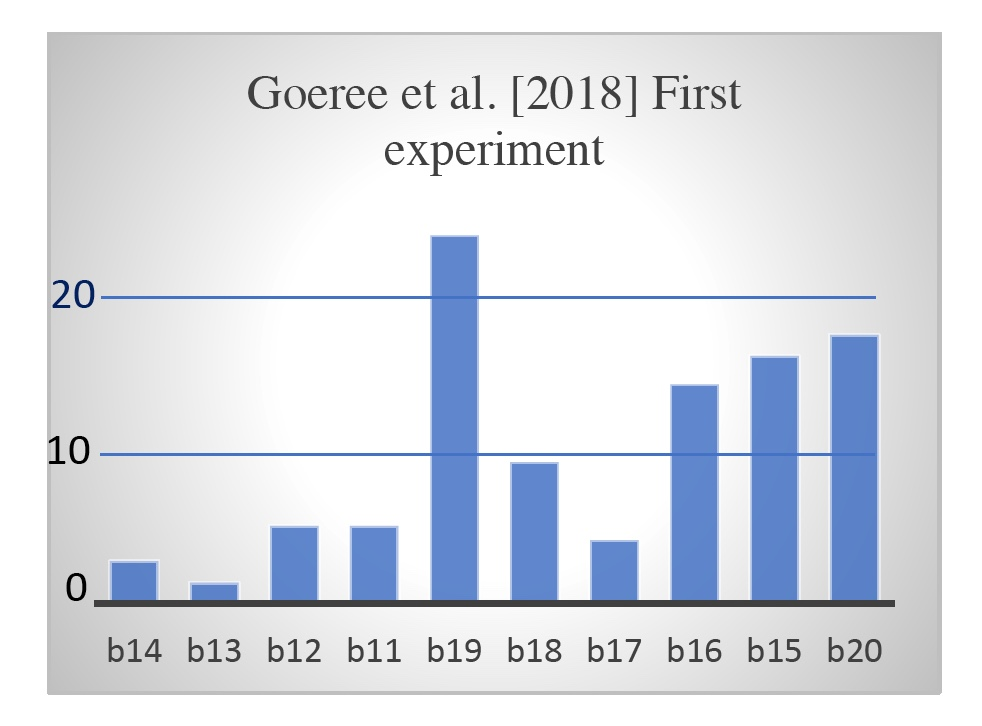
\includegraphics[height=5cm]{Articles-bons-a-composer/07_Umbhauer_en/07_Umbhauer_en_figures/Umbhauer_fig4a.jpeg}
    \label{fig:subfig1}%
  }
  \quad
  \subfloat[With the second arrangement]{%
    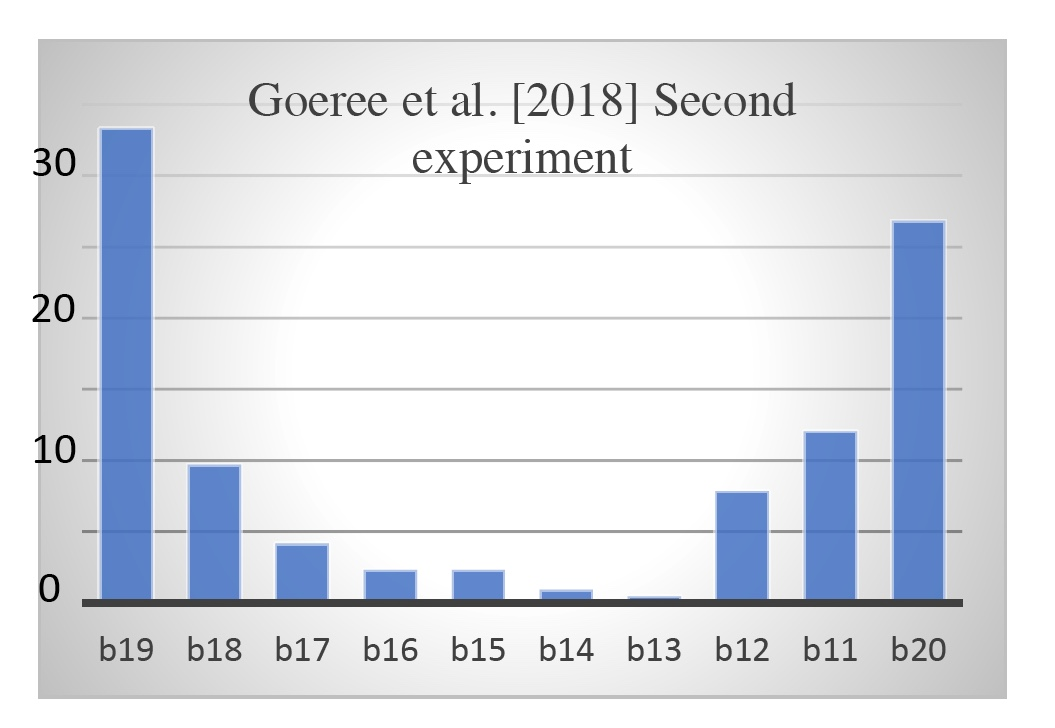
\includegraphics[height=5cm]{Articles-bons-a-composer/07_Umbhauer_en/07_Umbhauer_en_figures/Umbhauer_fig4b.jpeg}
    \label{fig:subfig2}%
  }
    \label{fig:mainfig}
\end{figure}

In both experiments there are players who behave like level-0, level-1
and level-2 players. In the first experiment, the percentages of players
choosing 20, 15 and 16 are larger than those choosing the other numbers
except for 19. In the second experiment the percentages of players
choosing 20, 11 and 12 are larger than those choosing the other numbers
except for 19 and 18. Yet, at the same time, first, there are very few
level-3 players in both experiments and the percentages of level-1,
level-2 and level-3 players are rather low: under 35\% in the first
experiment and under 21\% in the second, so these percentages are very
different from those obtained in AR's game (74\% in AR, 83\% in LR,
60.4\% in the Strasbourg classroom experiment). Second, 19 is the amount
most often played regardless of its rank in the level-\emph{k} process
(19 is the level-5 amount in the first experiment and the level-9 amount
in the second experiment). And even 18 is often played in both
experiments regardless of its rank in the level-\emph{k} process.
Finally, 20 is played much more often than in AR's game in both
experiments and especially in the second one (27\%). So, clearly, the
fact that large numbers lead to large sure payoffs, and the fact that 19
leads to the second largest sure payoff plus the opportunity to get the
bonus, play a main role.

GLZ showed how a common knowledge of noise in behavior can help us to
come closer to the observed distributions. MR also leads to behavior
that is closer to the experimental data. As regards MR, it is
interesting to observe that the mixed MR strategy is completely
unaffected by the order of the boxes (provided box 20 is the rightmost
box): so MR leads exactly to the same strategy in GLZ's games and in
AR's game. This is due to the fact that the regret structure is the same
in the three games. For example, the fact that 19 gives rise to the
payoff 39 when the opponent plays 18 (in both GLZ's experiments) leads
to a column of regrets that is the same as the column of regrets
obtained when the opponent plays 20 in AR's game. The fact that 15 gives
rise to the payoff 35 if confronted with an opponent playing 19 (first
experiment) and 14 (second experiment), leads to a column of regrets
that is exactly the same as the one obtained when the opponent plays 16
in AR's game. And so on. So minimizing regrets leads exactly to the same
constraints (only the order of the constraints changes). It derives from
this fact that MR leads to the probability distribution in figure 2. Of
course, this time, the mixed MR strategy does not look like the outcome
distribution obtained with level-\emph{k} players (when the percentage
of level-\emph{k} players decreases in \emph{k}). But MR fits with the
two main results obtained in GLZ's experiments. First, MR assigns
probability 0.25 to 19, a probability that is similar to the percentages
obtained in GLZ's experiments (24\% in the first experiment, 33\% in the
second experiment). Second, the total probability assigned to 18, 19 and
20 by MR is 0.7, a probability that is similar to the sum of percentages
on 18, 19, 20 in GLZ's experiments (51\% in the first experiment and
70\% in the second experiment).

Let us add a few words on NE and risk aversion. MR exploits the cautious
side of large amounts (namely 19), in addition to the regret of not
getting the bonus. \textcite{li2018} exploit the cautious side of 19
and 20 too; they work with the NE and show how the NE can also come
close to the experimental outcome distribution, when taking into account
the notion of risk aversion. So they show that the concave utility
function \(1 - e^{- 0.15x}\), where \emph{x} is the chosen amount, leads
to a NE that better fits with their experimental data, in that it
increases the probabilities on 18, 19 and 20. This is right, yet this
does not mean that the mixed NE is well suited to explain the player's
behavior. So it is worth observing that a function \(1 - e^{- ax}\),
with \(a > 0\), gives rise to a Nash equilibrium that behaves like the
usual (risk-neutral) NE: when the numbers played at equilibrium go from
\emph{x} to 20, the probability assigned to each number from \(x + 1\)
to 20 decreases in this number, the probability on \(x\) being the
complement to 1. Yet from a behavioral point of view, it seems rather
strange that \(x + 1\ \)is played with the largest probability and that
\(x - 1\ \)is played with probability 0. In fact, by definition, in a
mixed NE, a player's probabilities only have to stabilize (optimize) the
behavior of the other players. So in AR's game, they only have to ensure
that the opponent always gets 20 with all the amounts he plays with
positive probability: this is usually not the aim of the players in the
experiments.


\section{Conclusion}
\label{section:Conclusion_Umbhauer_en}

Arad and Rubinstein's 11--20 money request game is a very rich game that
triggers more nuanced behavior than level-\emph{k} reasoning.

Level-\emph{k} behaviors, especially level-1, level-2 and level-3
behaviors, are observed in the experiments. In the Strasbourg classroom
experiment, level-\emph{k} reasoning is clearly a main component of the
reasoning among the numerous students (32.4\%) playing 17 and 18. Most
of the students playing 18 exclusively engage in level-2 reasoning, and
60\% of the students playing 17 exclusively engage in level-3 reasoning.
Nearly half of the 5.8\% of students playing 16 even engage in level-4
reasoning.

But minimizing regrets plays an important role too. Let us here stress
an important difference between the 11--20 money request game and the
guessing game, the game used most often to study level-\emph{k}
reasoning. In a guessing game, to be the winner (to get 1), a player has
to do one additional step of reasoning in comparison with the depth of
reasoning of the others. Otherwise he gets 0, the losers' payoff. This
is clearly not the case in AR's game, where a player can get a nice
payoff without guessing anything. Playing 20 leads to the sure and large
payoff 20, regardless of the opponent. In the classroom experiment, if
we calculate the mean payoff of each strategy confronted by all played
strategies, 20 leads to the 4\textsuperscript{th} best expected payoff
(see figure 5). And the level-1 amount 19 leads to the second-best
payoff. This largely explains that the students in Strasbourg who play
19 and 20 generally do not justify their behavior with level-\emph{k}
reasoning. As already said above, the main argument justifying the play
of 19 fits with MR: ``By playing 19, I get 19 for sure, which is not far
from 20, and I keep the opportunity to get 39 by meeting a student who
plays 20.''


\begin{figure}[h]
    \centering
    \caption{Mean payoff associated with each requested amount}
    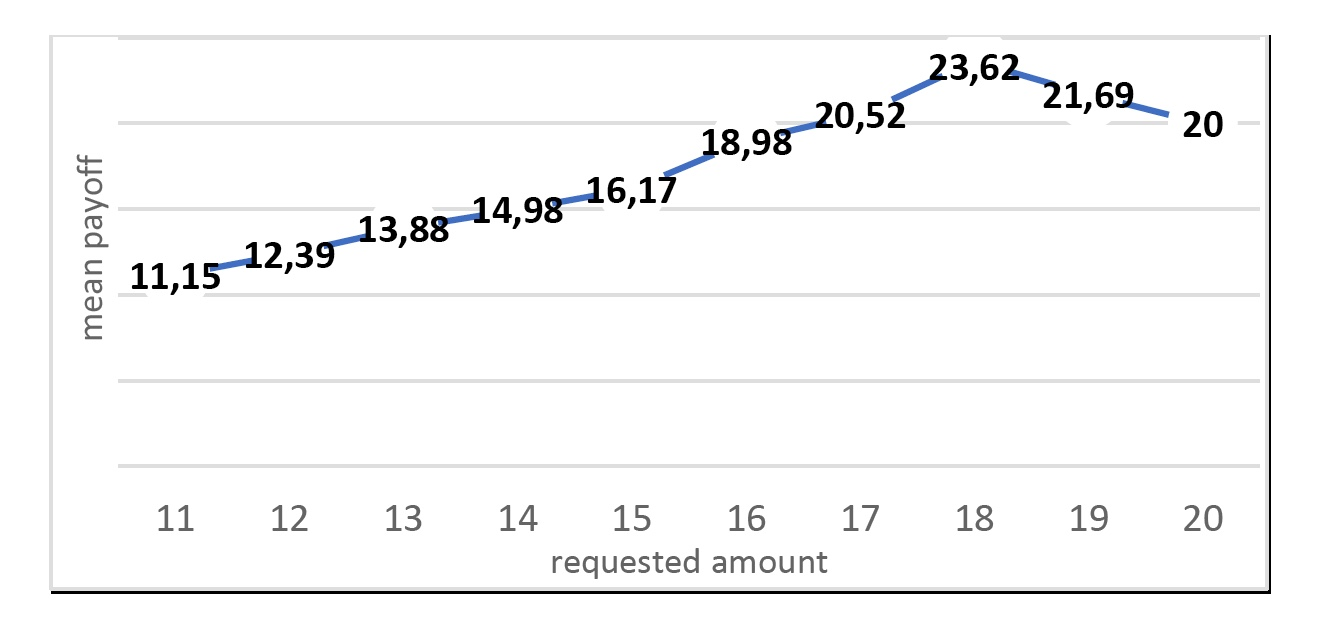
\includegraphics[height=5cm]{Articles-bons-a-composer/07_Umbhauer_en/07_Umbhauer_en_figures/Umbhauer_fig5.jpeg}
\end{figure}


We end the paper by shedding light on some particularities of the
Strasbourg classroom experiment, which are perhaps linked to the fact
that the students had the normal form matrix at their disposal. This
matrix helped them to compare their payoff with the opponent's one in
any possible configuration. And this may explain some behaviors that
have nothing to do either with level-\emph{k} reasoning or regret
minimization.

Thus, many students in Strasbourg, 8.3\%, play 11, just because they do
not want to offer the opponent the opportunity to get the bonus. It is
well known that the fear of not getting something (here the bonus) often
triggers the wish that others do not get it either. And playing 11 is
the only way to impede the opponent from getting the bonus. By playing
11, some students also want to minimize the maximal possible difference
(in their disadvantage) between their payoff and the opponent's one. In
fact, if a player plays 11, the opponent gets at best 9 units more, by
contrast to the 19 possible units if he plays another amount.

In a less extreme (and quite opposite) way, students who play 19,
respectively 20, sometimes justify their play by observing that they get
more than their opponent in all situations except for one (when the
opponent plays 18, respectively 19). That is to say, a student who plays
19 gets a larger payoff than the opponent when the opponent plays 20 or
a number from 11 to 17, and he gets less than the opponent only if the
latter plays 18. So he is better off than the opponent in 8
configurations (among 10). The same is true for a player who plays 20.
And it can be observed that, from 18 to 11, the lower the amount a
student plays, the lower is the number of configurations in which he
gets more than his opponent: with 18 he is better off than his opponent
in 7 configurations, with 11 he is better off than his opponent in 1
configuration. The fact that many students attribute more weight to the
difference in payoffs than the payoff they get is surely linked to their
experience of everyday life. Many of them have taken competitive
examinations where the objective is to achieve better scores than the
others.

AR's game, therefore, despite its simplicity, generates contrasting ways
of playing: it is revealed to be richer than expected by its authors.

\vspace{1cm}

\printbibliography


\begin{appendices}

\section{Proof of Proposition 1}
\label{Annexe:Proof of Prop 1}

\emph{a}) We solve:
\[
\min_{z\ p_{11}\ldots p_{T}}z
\]
u.c.
\[
\sum_{i = 11}^{T}{(T - i)p_{i}} \leq z
\]
\[
0p_{11} + \sum_{i = 12}^{T}{(B + 11 - i)p_{i} \leq z} \tag{A1}
\]
\[
\sum_{i = 11}^{j - 2}{(B + j - 1 - i)p_{i} + 0p_{j - 1} + \sum_{i = j}^{T}{(B + j - 1 - i)p_{i} \leq z}} \quad \text{ \emph{j} from 13 to } T
\]
\[
\sum_{i = 11}^{T}{p_{i} = 1}
\]
\[
p_{i} \geq 0 \quad \text{ \emph{i} from 11 to } T.
\]
We suppose that only \emph{p\textsubscript{i}}, with \(i \geq \ T - n\),
is strictly positive, with \emph{n} defined by
\(\frac{n(n + 1)}{2} < B < \frac{(n + 1)(n + 2)}{2}\).

Given the structure of the regret matrix, this implies that the regrets
associated with the columns \emph{j}, with \(j < T - n\), are strictly
lower than \emph{z}. This follows from the structure of the lines. In
line \emph{k}, the regrets are increasing in \emph{j}, with \emph{j}
from 11 to \emph{k}. So, given that we set \emph{p\textsubscript{i}} = 0
for \emph{i} from 11 to \(T - n - 1\), the only lines that matter are
those with \(k \geq T - n\). In all those lines, the regrets are
increasing in the column \emph{j}, with \emph{j} from 11 to \(T - n\),
which induces that the regret associated with column \emph{j}, with
\emph{j} from 11 to \(T - n - 1\) is strictly lower than \emph{z}.

We turn to the Karush Kuhn Tucker (KKT) function,
\[z + \sum_{j = 11}^{T}{\lambda_{j}(Regret(j) - z)} - \sum_{i = 11}^{T}{\mu_{i}p_{i} + \lambda\left( \sum_{t = 11}^{T}p_{t} - 1 \right)},\]
where $Regret(j)$ is the regret associated with column \emph{j}.

Given the assumption on the optimal \emph{p\textsubscript{i}} and the
consequences on the regrets, the multipliers \(\lambda_{j}\) for
\emph{j} from 11 to \(T - n - 1\) have to be null, the multipliers
\(\lambda_{j}\) for \emph{j} from \(T - n\ \)to \emph{T} have to be
positive or null, the multipliers \emph{µ\textsubscript{i}} have to be
null for \emph{i} from \(T - n\) to \emph{T}, and they have to be
positive or null for \emph{i} from 11 to \(T - n - 1\).

The derivative of the KKT function in \emph{z} leads to \(1 - \sum_{j = 11}^{T}\lambda_{j} = 0\), hence \(1 - \sum_{j = T - n}^{T}\lambda_{j} = 0\).

More generally the derivatives in \emph{p\textsubscript{i}} for \emph{i}
from 11 to \emph{T} are:
\[
(T - 11)\lambda_{11} + 0\lambda_{12} + \sum_{j = 13}^{T}{(B + j - 12)\lambda_{j}} - \mu_{11} + \lambda = 0
\quad \text{for} \: i = 11
\]
\begin{equation*}
\begin{split}
(T - i)\lambda_{11} + \sum_{j = 12}^{i}{(B - 1 + j - i)\lambda_{j} + 0\lambda_{i + 1} + \sum_{j = i + 2}^{T}{(B - 1 + j - i)\lambda_{j}}}\\
{-\: \mu_{i} + \lambda = 0} \quad \text{for \emph{i} from 12 to} \: T - 2  
\end{split}
\end{equation*}
\[
\lambda_{11} + \sum_{j = 12}^{T - 1}{(B + j - T)\lambda_{j} + 0\lambda_{T} - \mu_{T - 1} + \lambda = 0} \quad \text{for} \: i = T - 1
\]
\[
\sum_{j = 12}^{T}{(B - 1 + j - \ T)\lambda_{j} - \mu_{T} + \lambda = 0}
\quad \text{for} \: i = T.
\]

Subtracting the equations 2 by 2, starting from the last two ones, leads
to:
\[1 - \mu_{T - 1} = B\lambda_{T} - \mu_{T}\]
\noindent and
\[1 + B\lambda_{i + 2} - \mu_{i} = \ B\lambda_{i + 1} - \mu_{i + 1}\]
for \emph{i} from 11 to \(T - 2\).

$\mu_i = 0$ for \emph{i} from \(T - n\) to \emph{T}, and
\emph{n} is at least equal to 5, given that \(B \geq T > 11 + n\) and
\(n(n + 1)/2 < B < (n + 1)(n + 2)/2\). So we get
\(\lambda_{T} = \frac{1}{B},\ \lambda_{T - 1} = \frac{2}{B}\) and more
generally \(\lambda_{j} = \frac{(T + 1 - j)}{B}\) for \emph{j} from
\(T - n + 1\) to \emph{T}, with \(\lambda_{T - n + 1} = \frac{n}{B}\).
And
\(\lambda_{T - n} = 1 - \sum_{j = T - n + 1}^{T}\lambda_{j}{= 1 - \frac{n(n + 1)}{2B}.}_{}\)

Then we have \(1 + B\lambda_{T - n + 1} - \mu_{T - n - 1} = \ B\lambda_{T - n} - \mu_{T - n}\), i.e. \(1 + n - \mu_{T - n - 1} = B - n(n + 1)/2\).

So \(\mu_{T - n - 1} = 1 + n - B + \frac{n(n + 1)}{2} = \frac{(n + 1)(n + 2)}{2} - B > 0\)
by definition of \emph{n.}

Then we have \(1 + B\lambda_{T - n} - \mu_{T - n - 2} = \ B\lambda_{T - n - 1} - \mu_{T - n - 1}\), i.e. \(\mu_{T - n - 2} = 1 + B\lambda_{T - n} + \mu_{T - n - 1} = 2 + n\) and
\(\mu_{i} = \ 1 + \mu_{i + 1} = T - i\) for \emph{i} from 11 to
\(T - n - 3\), because \emph{λ}\textsubscript{j} = 0 for \emph{j} from 11 to
\(T - n - 1\).

We now turn back to the equations
\[\sum_{i = 11}^{j - 2}{(B + j - 1 - i)p_{i} + 0p_{j - 1} + \sum_{i = j}^{T}{(B + j - 1 - i)p_{i} = z}}\]
for \emph{j} from $T-n$ to \emph{T}.\footnote{If $T - n~= 12$ we
  have to add the equation \(0p_{11} + \sum_{i = 12}^{T}{(B + 11 - i)p_{i} \leq z}\) but this does not change the results.}

We want \emph{p\textsubscript{i}} = 0 for \emph{i} from 11 to
\(T - n - 1\). Subtracting the equations 2 by 2, starting from the first
two ones, leads to : \(1 + Bp_{j - 1} = Bp_{j}\) for \emph{j} from
\(T - n\) to \(T - 1\).

Given that we want \emph{p\textsubscript{i }}= 0 for \emph{i} from 11 to
\(T - n - 1\), it follows \(p_{T - n} = \frac{1}{B}\) and more generally
\(p_{T - n + i} = \frac{i + 1}{B}\ \) for \emph{i} from 0 to \(n - 1\)
and \(p_{T} = 1 - \frac{n(n + 1)}{2B}\).

Given the structure of the equations (1), the nullity of
\emph{p\textsubscript{i}} for \(i < T - n\) immediately ensures that
\(\sum_{i = 11}^{j - 2}{(B + j - 1 - i)p_{i} + 0p_{j - 1} + \sum_{i = j}^{T}{(B + j - 1 - i)p_{i} < z}}\)
for \(j < T - n\), and therefore justifies the nullity of the
\emph{λ\textsubscript{j}}, for \emph{j} from 11 to \(T - n - 1\).

So, given the convexity of the optimization problem, \(p_{i} = 0\) for
\emph{i} from 0 to \(T - n - 1\), \(p_{T - n + i} = \frac{i + 1}{B}\ \)
for \emph{i} from 0 to \(n - 1\) and \(p_{T} = 1 - \frac{n(n + 1)}{2B}\)
is the solution of the optimization program.

The proof of part~\emph{b} (\(B = n(n + 1)/2\)) is similar as regards the
two probability distributions given in proposition 1, and the convexity
of the solution set follows from the convexity of the problem.

\emph{c}) Given that
\(\sum_{i = T - n}^{T}{(B + T - n - 1 - i)p_{i} = z}\), we have

\[z = \sum_{i = 1}^{n}{\frac{(B - i)i}{B} + (B - n - 1)\left( 1 - \frac{n(n + 1)}{2B} \right)}\]

\[= B - \sum_{i = 1}^{n}{\frac{i^{2}}{B} + \frac{n(n + 1)^{2}}{2B} - (n + 1) = B + \frac{n(n + 1)(n + 2)}{6B} - (n + 1)}\]

By construction this regret is lower than \(B - 1\) (the regret obtained
with the pure strategies \emph{B} and \(B - 1\)); it can be checked that
\emph{z} is strictly lower than \(B - 1\) given the definition of
\emph{n}.

\section{Proof of Proposition 3}
\label{Annexe:Proof of Prop 3}

\emph{a}) We have \(z = B - (n + 1) + \frac{n(n + 1)(n + 2)}{6B}\).

The expected payoff can be calculated as follows. For each number chosen
by the opponent the mean payoff obtained by a player is the best reply
payoff to the opponent's amount minus \emph{z}, by construction of
\emph{z}.

As a matter of fact, when player 2 plays an amount \emph{y} in the
support of the MR strategy, then player 1, when he plays the amount
\emph{x} (in the support of the MR strategy), gets \(\ (y - 1 + B)\ –\)
\(r_{1}(x,y)\)

Hence, given that player 1 plays \emph{x} with probability
\emph{p\textsubscript{x}}, his mean payoff when player 2 plays \emph{y}
is
\[\sum_{x = T - n}^{T}{p_{x}(y - 1 + B - r_{1}(x,y))}=y - 1 + B - \sum_{x = T - n}^{T}{p_{x}r_{1}(x,y)} = y - 1 + B - z\]
by construction of \emph{z}. So, given that the opponent chooses each
amount \emph{y} with probability $p_y$, the expected payoff of a
player is simply:
\[
\sum_{y = T - n}^{T}{p_{y}(y - 1 + B - z)} =  \left( \sum_{y = T - n}^{T}{p_{y}(y - 1 + B)} \right) - z.
\]
It follows from the above that the expected MR payoff is just the mean
best reply payoff minus \emph{z}. So we get:
\begin{equation*}
\begin{split}
\frac{1}{B}.\ (B + T - n - 1) +& \frac{2}{B}.(B + T - n + 1 - 1) + \ldots + \frac{n}{B}.(B + T - n - 2 + n)\\
&+ \frac{\left( B - \frac{n(n + 1)}{2} \right)}{B}.\ (B + T + n - n - 1) - z\\
&= (B + T - n - 2 - z) + \sum_{i = 1}^{n} \frac{i^{2}}{B} + \frac{(n + 1)\left( B - \frac{n(n + 1)}{2} \right)}{B}\\
&= T + n - \frac{n(n + 1)(n + 2)}{3B}.
\end{split}
\end{equation*}

Given that \(n(n + 1)/2 < B < (n + 1)(n + 2)/2\), this payoff is between
\(T + (n - 4)/3\) and \(T + n/3\).

\emph{b}) We know that if player 2 plays \emph{y} in the support of the mixed MR
  strategy, player 1 gets \(y - 1 + B - z\), i.e.
  \(y + n - \frac{n(n + 1)(n + 2)}{6B}\). So the maximal mean payoff
  player 1 can get is \(T + n - \frac{n(n + 1)(n + 2)}{6B}\).

If player 2 plays \(y = T - n\), the mean payoff
\(y + n - \frac{n(n + 1)(n + 2)}{6B}\) is also equal to
\(\sum_{x = T - n}^{T}{p_{x}x}\), because player 1 never gets the bonus.
Hence
\(\sum_{x = T - n}^{T}{p_{x}x} = T - n - 1 + B - z = T - \frac{n(n + 1)(n + 2)}{6B}\).

For \(y < T - n\), player 1's mean payoff is always
\(\sum_{x = T - n}^{T}{p_{x}x}\), so he gets
\(T - \frac{n(n + 1)(n + 2)}{6B}\), regardless of the value \emph{y}.

The other results follow from replacing \emph{B} by
\(\frac{n(n + 1)}{2}\) and \(\frac{(n + 1)(n + 2)}{2}\).


\end{appendices}

\end{refsection}

\end{Article}
